\section{Assessment}\label{section:assessment3}

Scalable assessment of assignments is a crucial requirement of tools to be employed in a large-scale e-learning context, such as a \mooc. Section~\ref{section:assessment2} presented \tool's scalable assessment strategy, which is based on automated execution of software tests and can provide learners with immediate and frequent feedback.

In order not to limit the capabilities and the value of assessment, we decided against imposing a homogeneous testing method. Instead, we allow instructors to use the testing framework that fits their requirements best.

\subsection{Workflow}

\begin{figure}
\centering
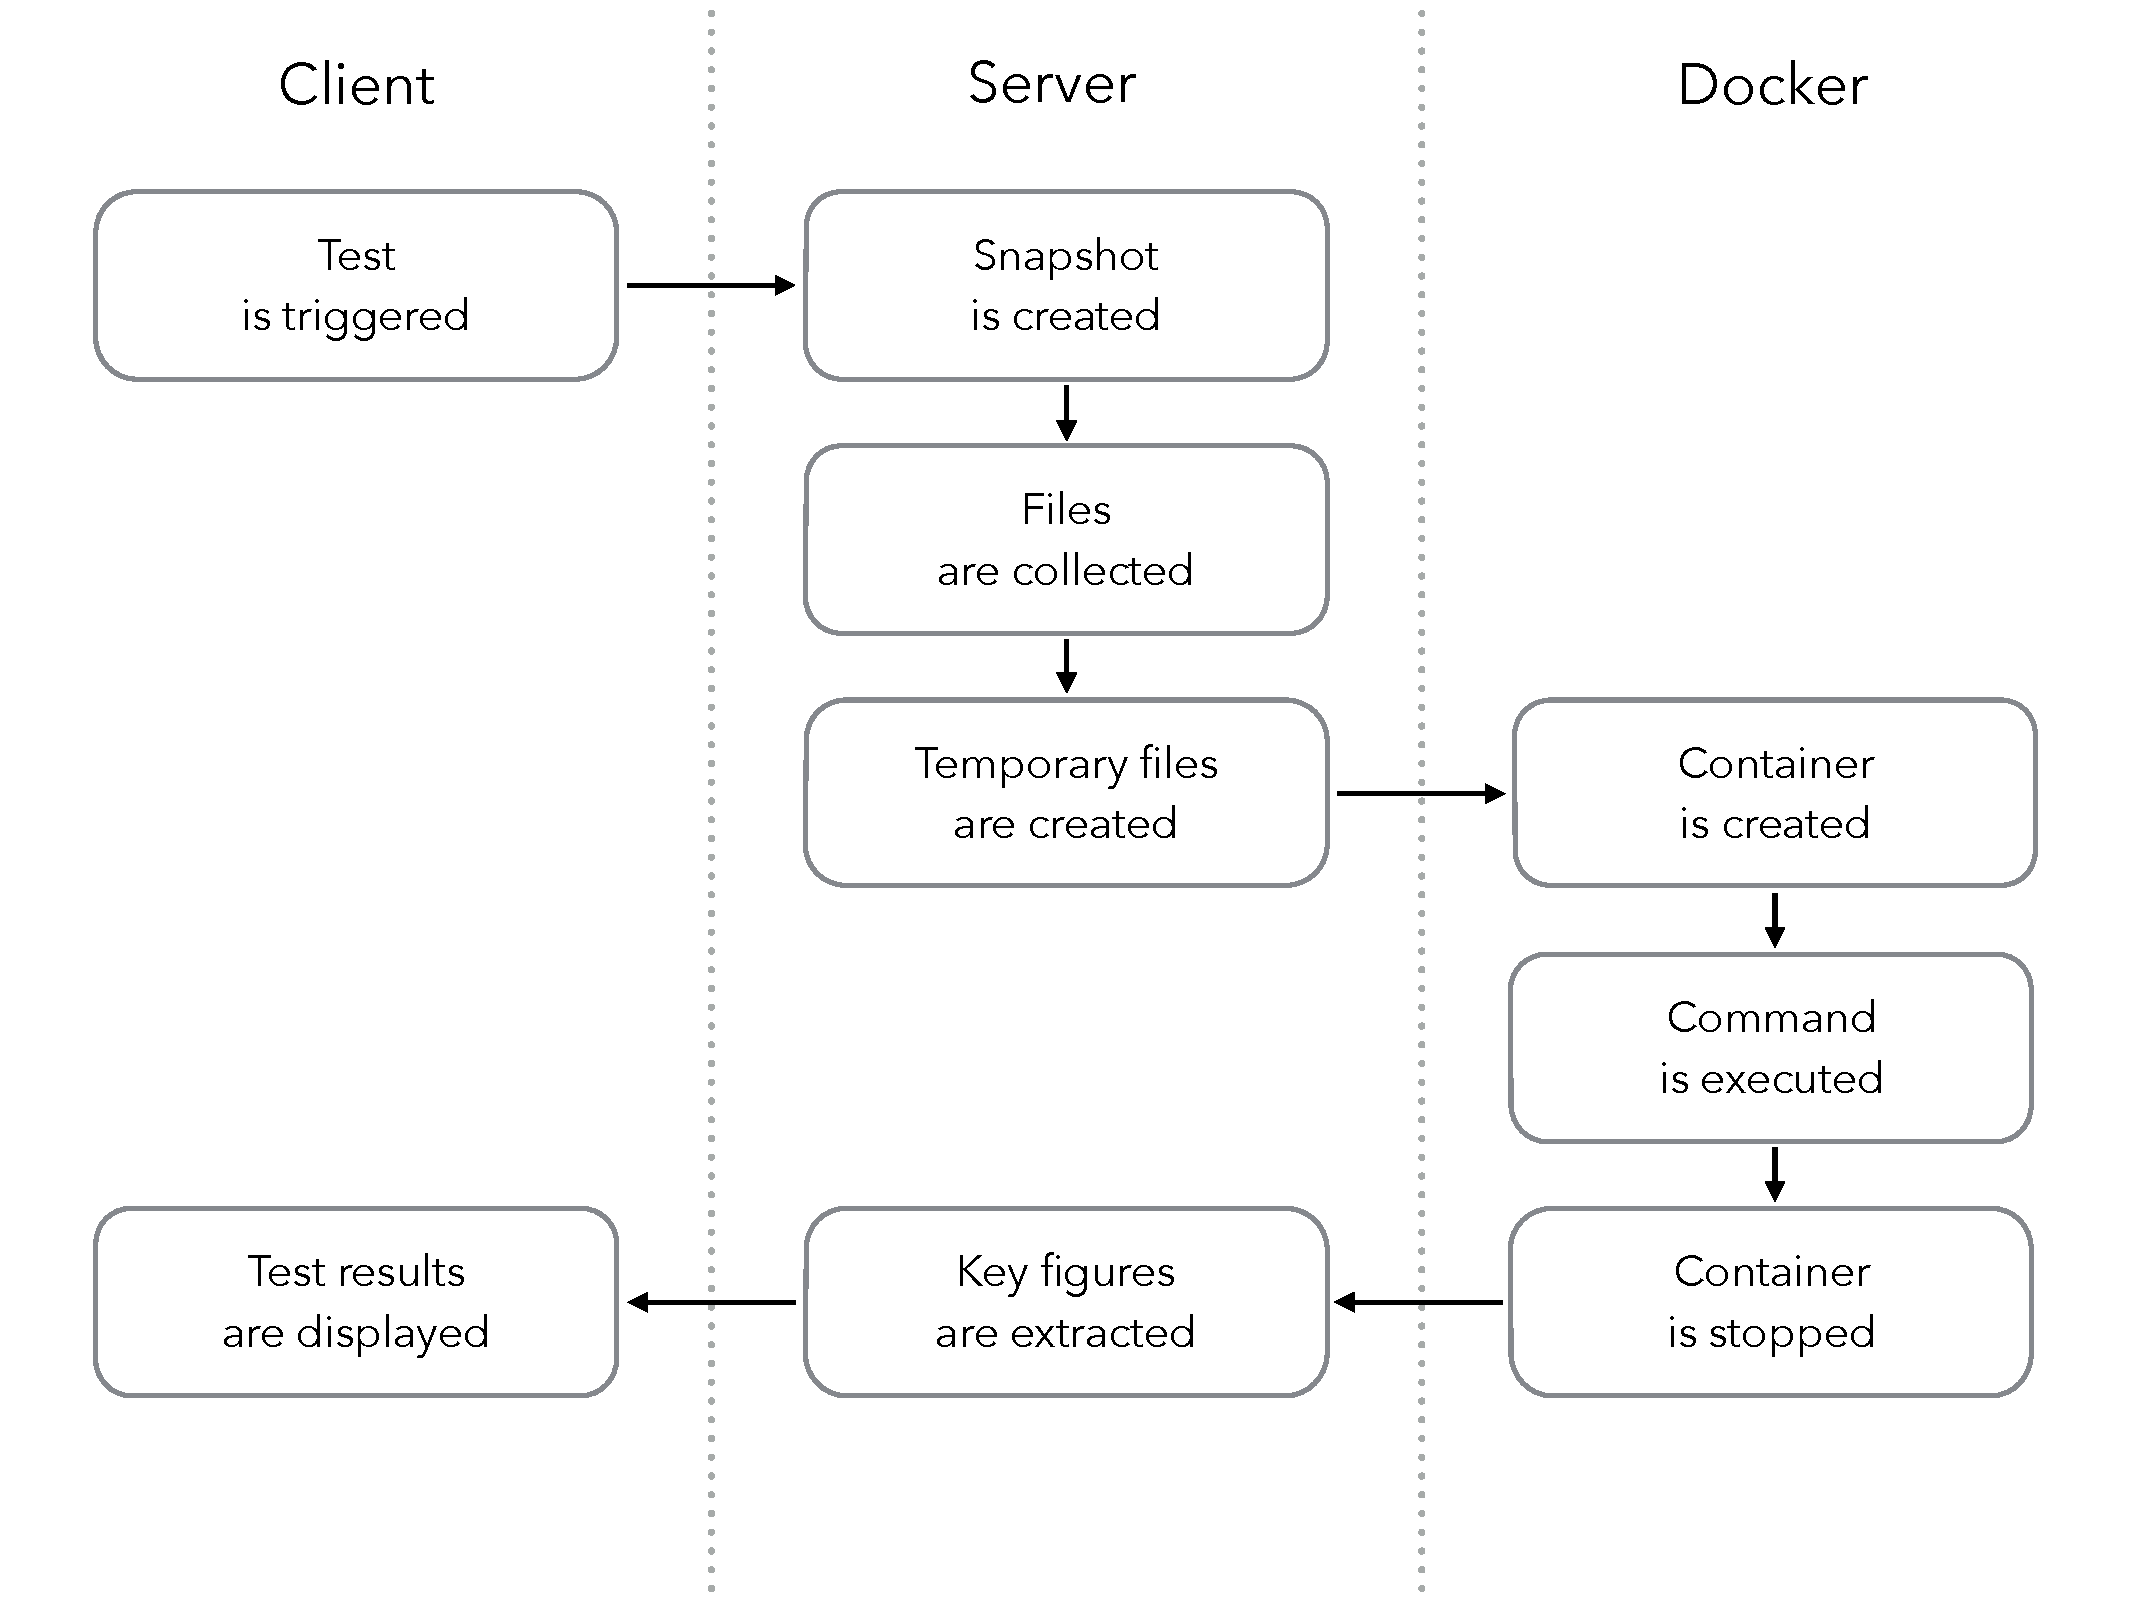
\includegraphics[clip=true, trim=0.5cm 3cm 0.5cm 0.5cm, width=\textwidth]{images/assessment}
\caption{Assessment Workflow}
\label{figure:assessment}
\end{figure}

\tool's assessment workflow is based on executing a learner's solution against a set of tests. Since these tests are invoked in the same manner as learners' main programs, the execution workflow, which is depicted in Figure~\ref{figure:assessment}, is very similar to that described in Section~\ref{section:code-execution2}.

Initially, an up-to-date code snapshot is created. After that, the learner's work, exercise skeleton files, and, most important, the exercise's tests are written to a temporary directory, which is supplied to a Docker container.

\begin{listing}
\inputminted[frame=lines]{sh}{listings/docker-run2.sh}
\vspace{-0.33cm}
\caption{Exemplary Docker Invocation for Assessing a Learner’s Code Submission}
\label{listing:docker-run2}
\end{listing}

Every test file is executed in a separate container based on the execution environment's Docker image. To do so, the execution environment's test command in invoked. Listing~\ref{listing:docker-run2} shows an exemplary invocation in Docker's \gls{cli} syntax using the example of the popular Ruby testing framework RSpec.

When the test runs are finished, test results are extracted from the testing framework's output. The final assignment score is calculated based on the single test files' weighted percentages of passed tests. Finally, the assessment results are displayed to the student.

\begin{figure}
\centering
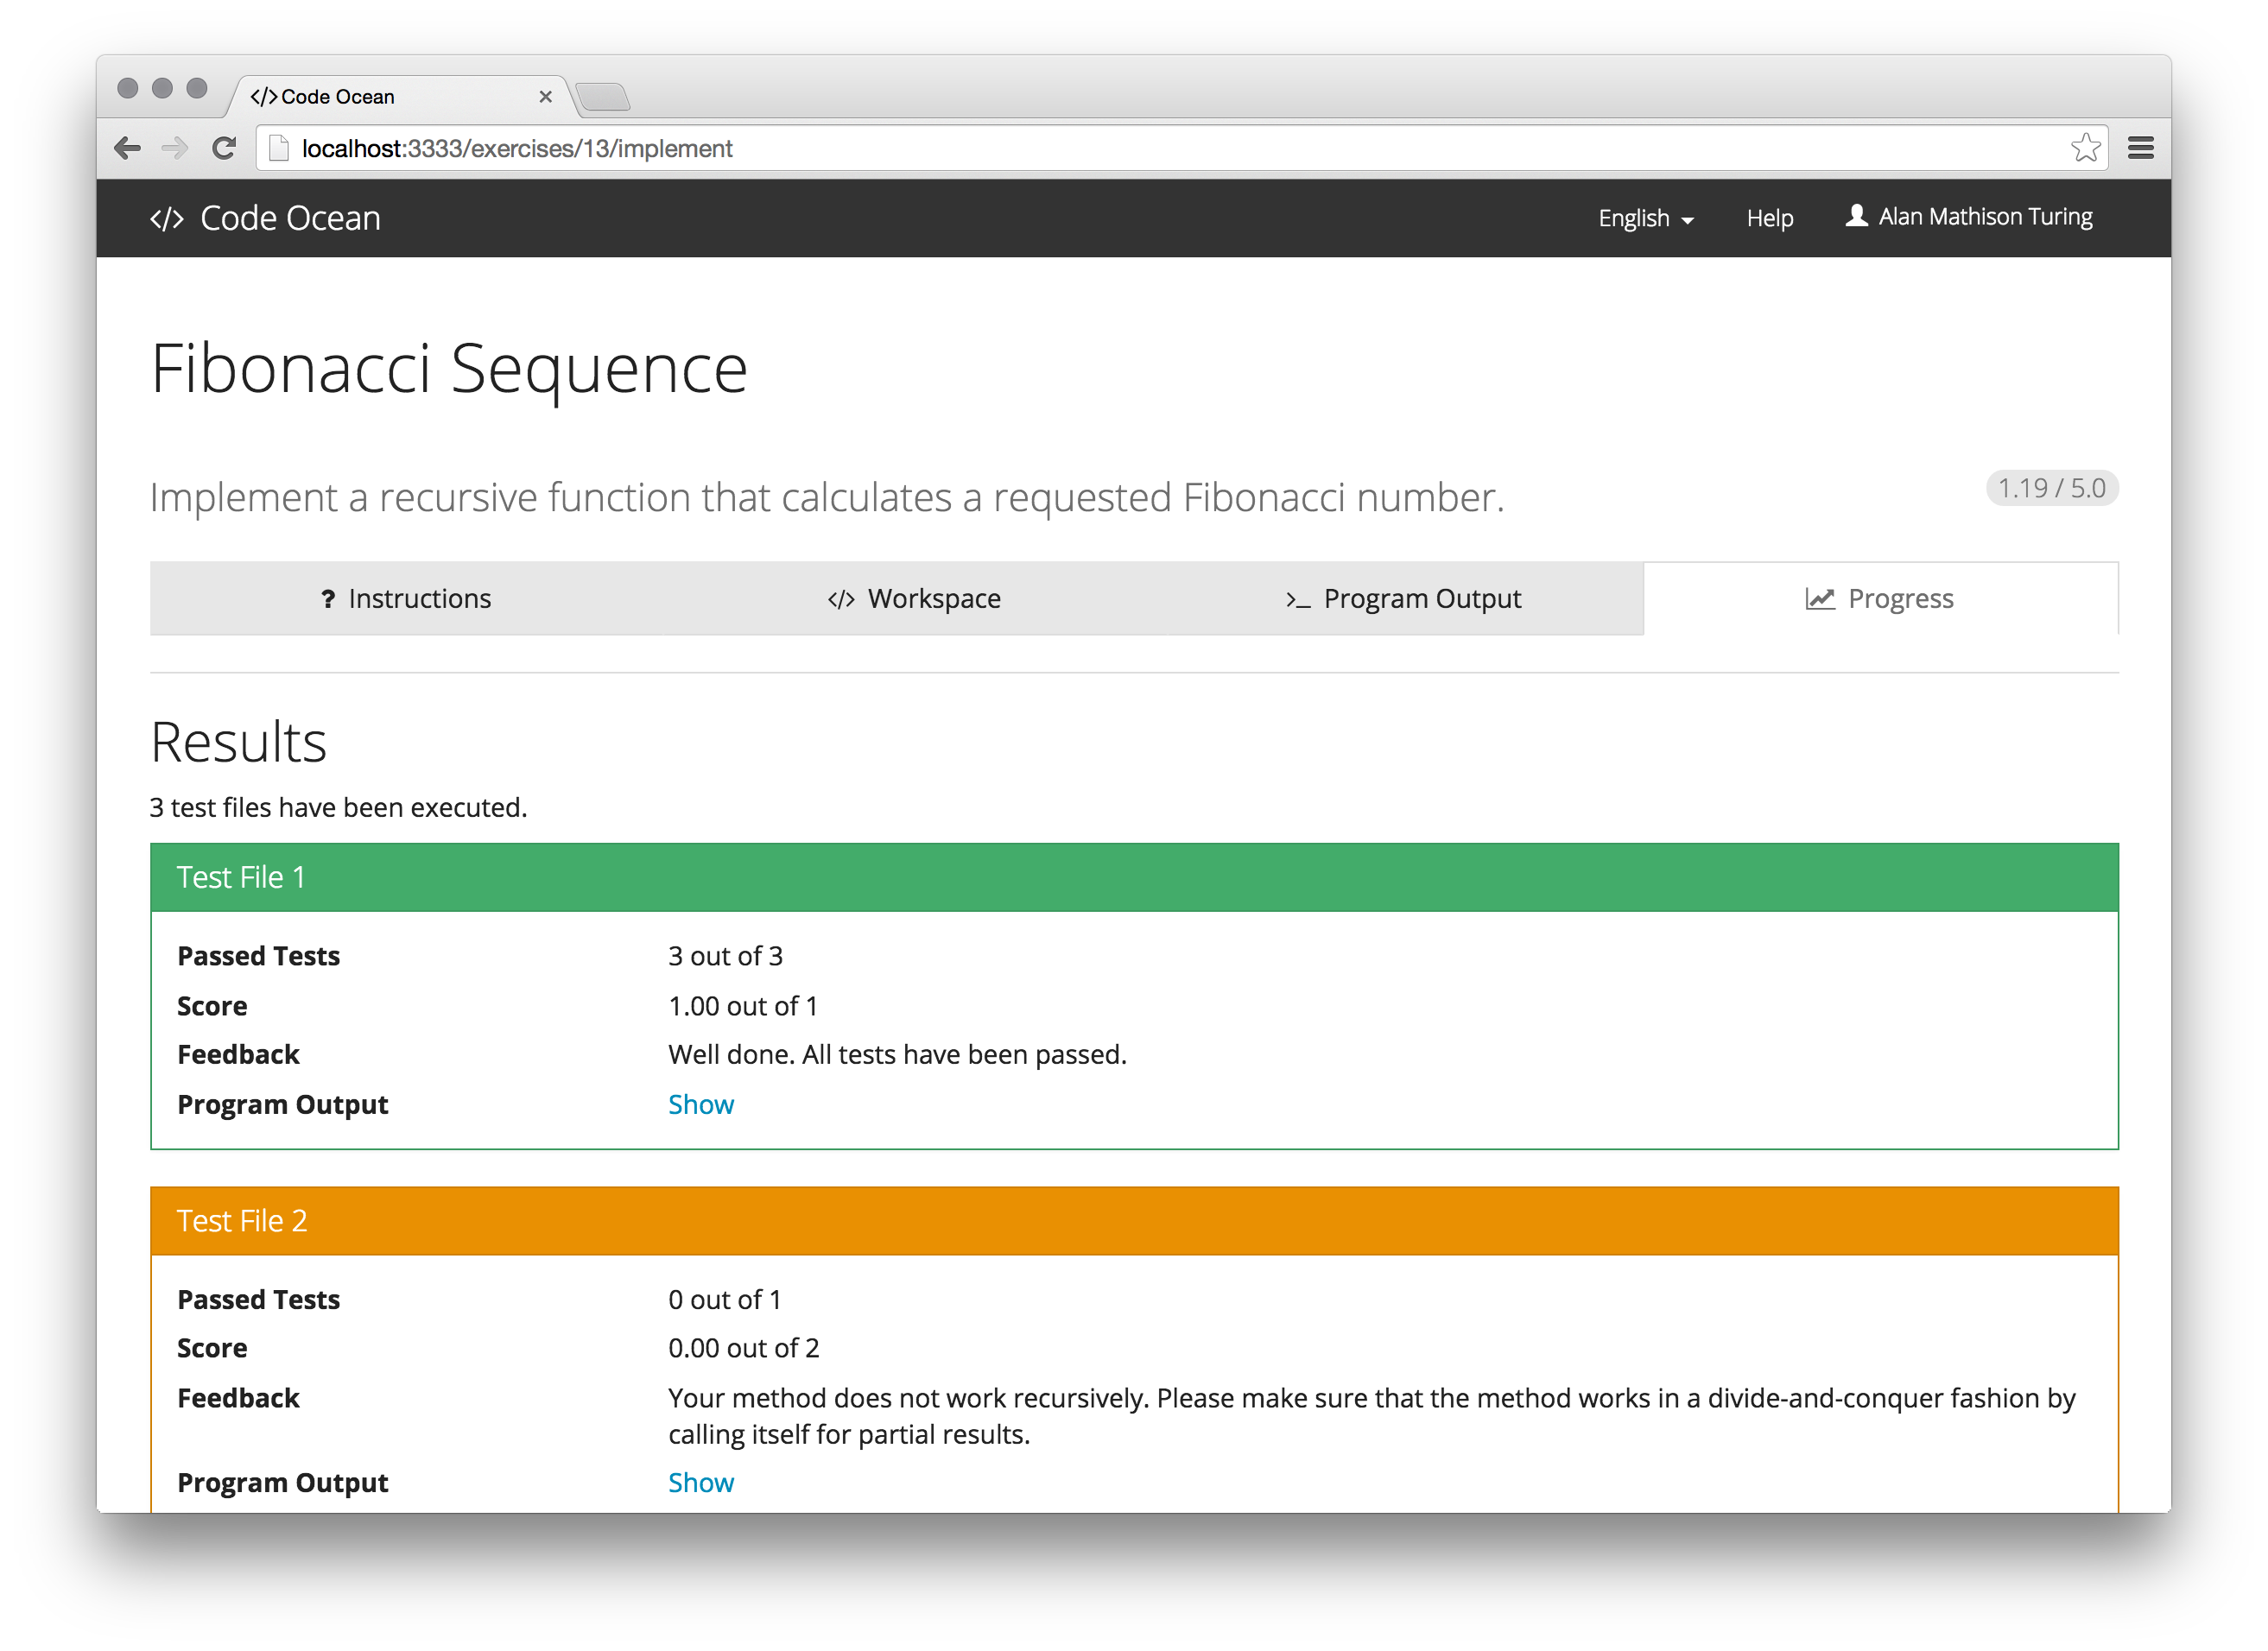
\includegraphics[width=\textwidth]{images/development-environment3.png}
\vspace{-1cm}
\caption{Development Environment: Assessment Presentation}
\label{figure:development-environment3}
\end{figure}

Figure~\ref{figure:development-environment3} depicts how assessment results are presented to the learner. The development environment's fourth tab contains the aggregated score of all test cases as well as detailed information per test file. For every file, the view displays the number of passed tests, the awarded score, and an instructor-provided feedback message if applicable.

The low-level testing framework output is presented in the adjacent tab. The output associated to a particular file can be accessed by following a link in the results overview. This allows students to form a connection between the teacher-provided feedback message and the low-level textual output.

\subsection{Metadata}

In order to control the weight of tests and to supply textual feedback, instructors need means to associate this kind of metadata with tests.

Since we decided to support a wide variety of testing frameworks, there is no universally applicable way of specifying metadata along with tests, for instance by using a \gls{dsl}~\cite{pieterse2013automated} or dedicated source code annotations~\cite{vihavainen2013scaffolding}.

Instead, instructors have to specify a test's metadata by means of attributes of the file containing the test (see Section~\ref{section:domain-model}). Therefore, in order to perform weighting and specify feedback in a fine-grained manner, a program's specification has to be expressed using multiple test files.

\subsection{Testing Framework Adapters}

In order to calculate a score and display it prominently in \tool's \gls{ui}, the application has to obtain key figures from the test run. Those are the number of executed test cases, the number of passed test cases, and the number of failed test cases.

Since we decided to provide teachers with the flexibility to use an arbitrary testing framework of their choice, there is no single source of data but a wide range of testing frameworks, each of which providing a proprietary \gls{api} and using a proprietary output format. In order to obtain the required key figures despite this inhomogeneity, \tool utilizes framework-specific adapters that extract the required information from testing frameworks' textual output. Such an adapter has to be provided for every testing framework or family of related frameworks to be used with \tool.

A testing framework adapter is a lean Ruby class that extends the generic \mintinline{rb}{TestingFrameworkAdapter} class and implements the \mintinline{rb}{parse_output} method in a framework-specific manner. Based on the testing framework configured for an execution environment, a specific testing framework adapter is instantiated as part of the test execution workflow. In the workflow's last step, the testing framework adapter is used to extract the key figures named above from the testing framework's textual output. For this purpose, the output is passed to the adapter's \mintinline{rb}{parse_output} method in order to be parsed. A testing framework adapter is expected to return a hash\foo{http://www.ruby-doc.org/core-2.1.5/Hash.html} including at least two of the three keys \emph{count}, \emph{failed}, and \emph{passed}. Unless included, the third key can be inferred from the two given ones.

\begin{listing}
\inputminted[frame=lines]{rb}{listings/rspec_adapter.rb}
\vspace{-0.33cm}
\caption{Testing Framework Adapter for RSpec}
\label{listing:rspec-adapter}
\end{listing}

\begin{listing}[h]
\inputminted[frame=lines]{text}{listings/rspec-output.txt}
\vspace{-0.33cm}
\caption{Output of an Exemplary RSpec Invocation, Using the Default Formatter}
\label{listing:rspec-output}
\end{listing}

Listing~\ref{listing:rspec-adapter} depicts \tool's testing framework adapter for RSpec. The single responsibility of the class is to parse RSpec-specific test output, as exemplarily depicted in Listing~\ref{listing:rspec-output}. According to the convention, the adapter extends the \mintinline{rb}{TestingFrameworkAdapter} class and implements the \mintinline{rb}{parse_output} method. It extracts the required key figures from the test output by means of a single regular expression that matches the number of executed tests and the number of failed tests.

As the example shows, testing framework adapters can be provided without much effort. Therefore, the set of testing frameworks supported by \tool is easily extensible.
